\documentclass{standalone}
\usepackage{tikz}
\usepackage{standalone}
\begin{document}
	
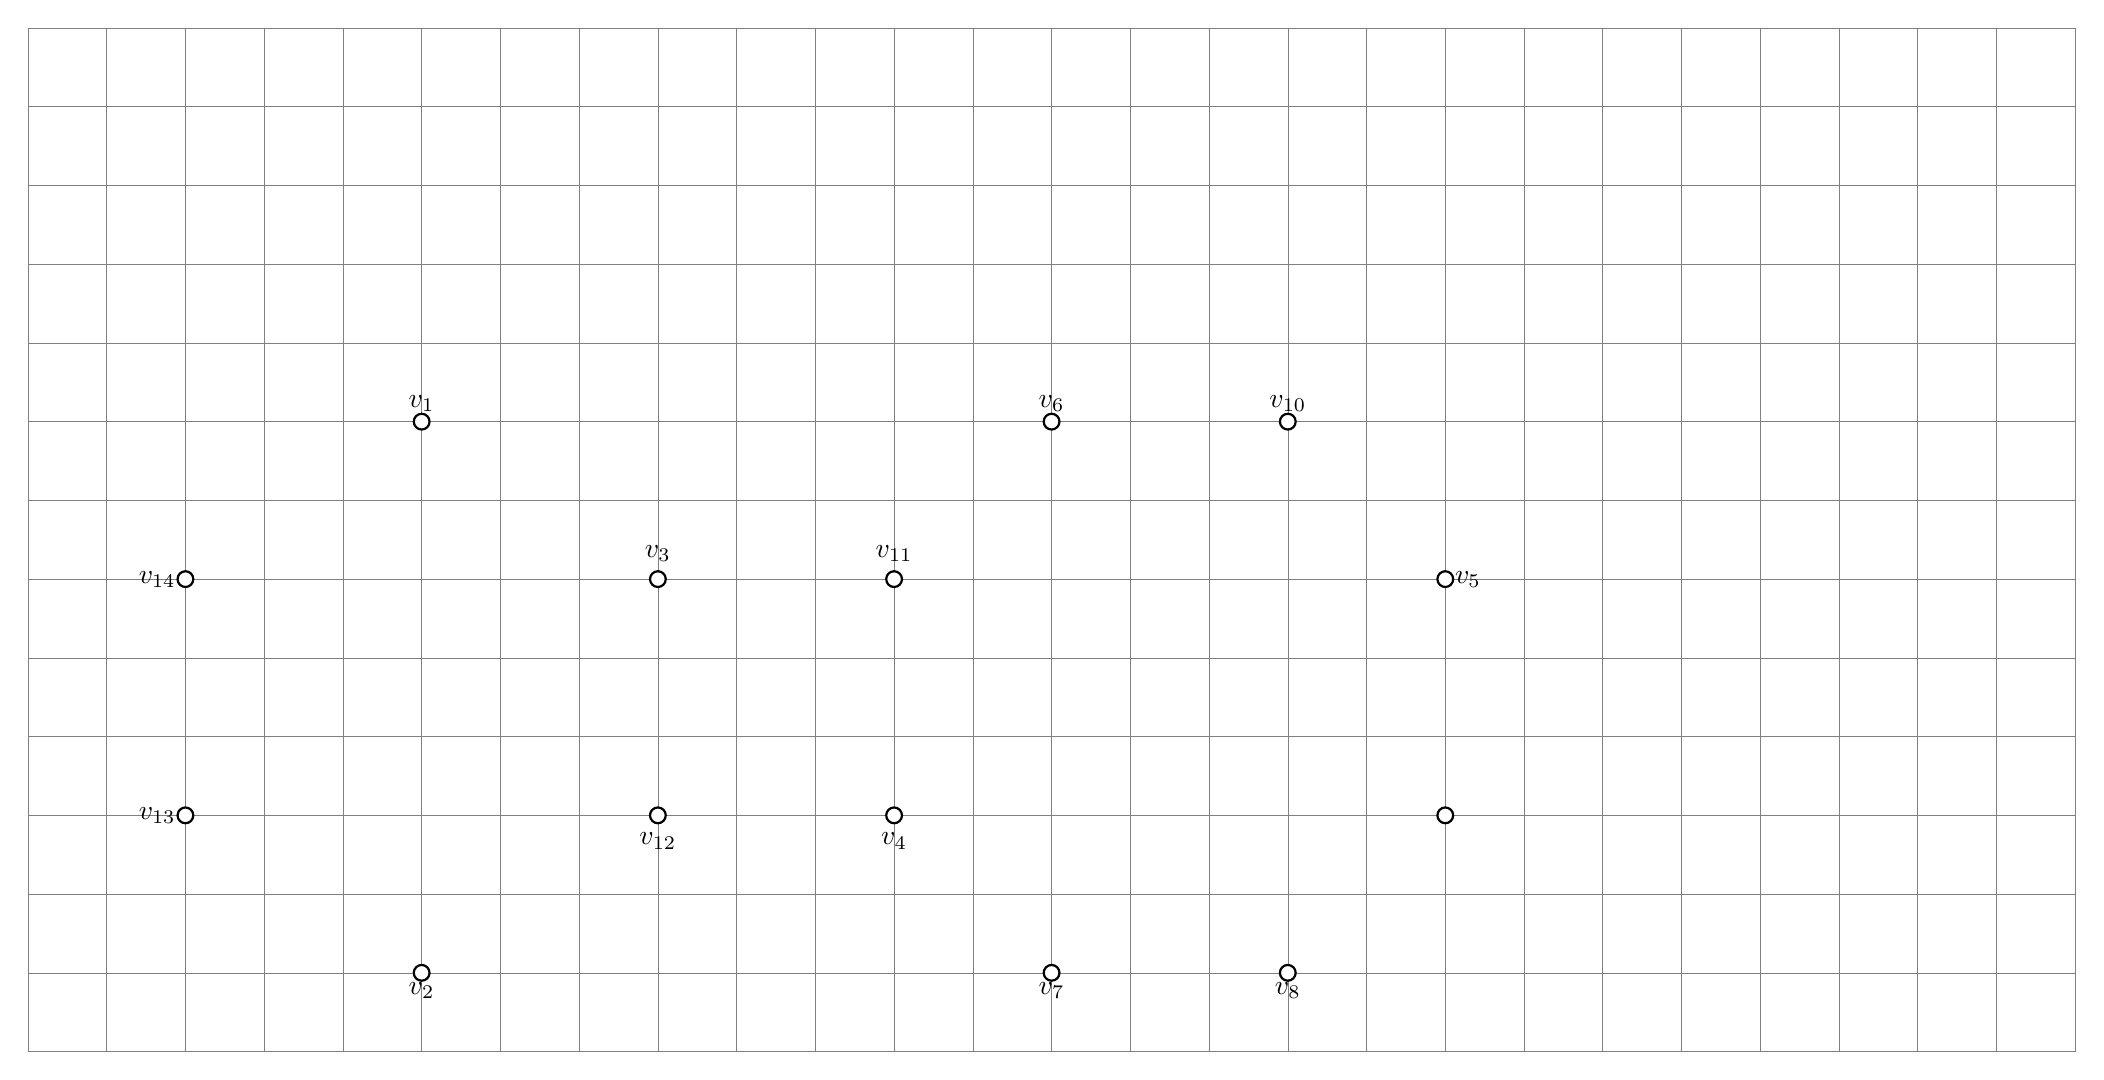
\begin{tikzpicture}
\draw [help lines] (-1,-1) grid (25, 12);


\draw [fill=white, thick] (4,0) circle [radius = 0.1];
\draw [fill=white, thick] (1,2) circle [radius = 0.1];
\draw [fill=white, thick] (7,2) circle [radius = 0.1];
\draw [fill=white, thick] (1,5) circle [radius = 0.1];
\draw [fill=white, thick] (7,5) circle [radius = 0.1];
\draw [fill=white, thick] (4,7) circle [radius = 0.1];

\draw [fill=white, thick] (10,2) circle [radius = 0.1];
\draw [fill=white, thick] (10,5) circle [radius = 0.1];
\draw [fill=white, thick] (17,2) circle [radius = 0.1];
\draw [fill=white, thick] (17,5) circle [radius = 0.1];
\draw [fill=white, thick] (12,0) circle [radius = 0.1];
\draw [fill=white, thick] (12,7) circle [radius = 0.1];
\draw [fill=white, thick] (15,0) circle [radius = 0.1];
\draw [fill=white, thick] (15,7) circle [radius = 0.1];

\node [below] at (4,0) {$v_2$};
\node [left] at (1,2) {$v_{13}$};
\node [left] at (1,5) {$v_{14}$};
\node [above] at (4,7) {$v_1$};
\node [above] at (7,5.1) {$v_3$};
\node [below] at (7,1.9) {$v_{12}$};

\node [below] at (15,0) {$v_8$};
\node [below] at (12,0) {$v_7$};
\node [below] at (10,1.9) {$v_4$};
\node [above] at (10,5.1) {$v_{11}$};
\node [above] at (12,7) {$v_6$};
\node [above] at (15,7) {$v_{10}$};
\node [right] at (17,5) {$v_5$};








\end{tikzpicture}
	
\end{document}
